\chapter*{Introduction}
\label{Introduction}
\addcontentsline{toc}{chapter}{\textbf{Introduction}}

\section*{The decline of global biological diversity : state of the world}
\addcontentsline{toc}{section}{The decline of global biological diversity : state of the world}

\label{intro:facts}
% Setting the stage : global decline
Nature has been deterioting for the past centuries, and much has already been lost \citep{ipbes_2022_6417333}. Across all the scales of analysis, the state of nature is critical. The structural conditions of ecosystems (e.g. interactions between biotic and abiotic elements that cause different structural phenomena and lead ecosystems to provide various resources, including wildlife habitat, carbon sequestration etc), the compositions (e.g. species richness\footnote{ Species richness measures the \textit{number of species} in a given period and location}) of ecological communities and populations (e.g. species abundance\footnote{ Species abundance measures the \textit{population of species} in a given period and location}) of species have experienced dramatic changes. 

Ecosystem structure forms the basis of natural and social-ecological processes: its disruption has far reaching consequences. Overall, only 13\% of oceans and 23\% of land remains sufficiently unimpacted by humanity to be classified as \textit{wilderness} \citep{jones_2018_location, watson_2016_catastrophic}. While deforestation has slowed since the 1990s, vegetation biomass (including trees) has dropped to below 50\% of the level expected absent human land-use, suggesting that a \textit{planetary boundary} has been crossed \citep{steffen_2015_planetary}. Additionally, anthropogenic climate change drives ecosystem disruptions on land \citep{conradi_reassessment_2024} and at sea \citep{gomes_marine_2024}, through changes various channels including ecological suitability and foodweb disturbances.





 At the global scale,n 

At the local scale, the average balance of gains and losses of psecies in locations across the world is 

At the local scale, species composition is changing rapidly. The average balance of gain and losses of species in locations across the world is debated and depends on the context \citep{thomas_2013_local}, due to local extinction, species migration and non-alien invasive species spread. Nonetheless, it appears that local communities are becoming more and more similar \citep{mckinney_1999_biotic}, driven by the increased extent of animal and plant non-alien invasive species, rising by 13\% per decade \citep{seebens_no_2017}. 

Finally, biological diversity, e.g. \textit{``the variability among living organisms from all sources including, inter alia, terrestrial, marine and other aquatic ecosystems and the ecological complexes of which they are part; [including] diversity within species, between species and of ecosystems''}\footnote{\href{https://www.cbd.int/convention/articles/default.shtml?a=cbd-02}{ Article 2  of the Convention on Biological Diversity}, 1992, in the wake of the Rio United Nations Conference on Environment and Development },  is threatened by a mass extinction, as the global rate of species extinction is at least ten times higher than the average rate over the past 10 million years and is accelerating \citep{barnosky_has_2011, ceballos_accelerated_2015}. On average, 25\% of species are currently threatened with global extinction (Figure \ref{fig:intro_iucn}, \cite{IUCN_redlist_2024}) across a wide range of plant and animal species, on land and at sea. Using different methods\footnote{ The IUCN Redlist uses detailed accounts for species, in a bottom-up approach, to analyze the extinction risk of species. A top-down approach, relying on the evolution of available habitat and the species-area relationship, uses changes in land use to forecast the extinction of species in a more aggregate manner \citep{Diamond1972BiogeographicKE}}, \cite{Hoskins309377} find that hundreds of thousands of plant and animal species are threatened, and will repay the \textit{extinction debt} caused by anthropogenic changes to their habitats : only 92.1\% of terrestrial vertebrate species, 91.6\% of terrestiral invertebrates and 90.7\% of terrestrial plants have enough habitat to persist. These results suggest that around half a million terrestrial animal and plant species - including over 3000 vertebrates and over 40,000 plants - \textit{dead species walking}, doomed to become extinct, unless their habitats improve in time to prevent it \citep{ipbes_2022_6417333}.
 
 \begin{figure}[H]
    \centering
    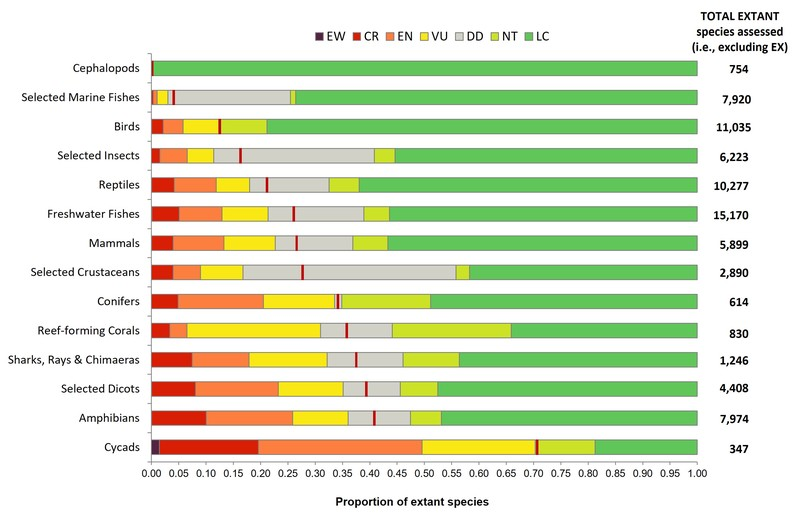
\includegraphics[width=0.8\linewidth]{figures/intro/IUCN_redlist}
    \caption{The proportion of extant (i.e., excluding Extinct) species in \citet{IUCN_redlist_2024}}
    \subcaption*{Assessed in each category for the more comprehensively assessed (i.e., at least 80\% of the group has been assessed) groups containing $\geq$ 150 species. Species are grouped into classes (with the exception of reef-forming corals, which includes species from classes Anthozoa and Hydrozoa), and are ordered according to the vertical red lines, which indicate the best estimate for proportion of extant species considered threatened (CR, EN, or VU) or Extinct in the Wild (EW). The numbers to the right of each bar represent the total number of extant species assessed for each group. \textbf{EW} - Extinct in the Wild, \textbf{CR} - Critically Endangered,\textbf{ EN} - Endangered, \textbf{VU} - Vulnerable, \textbf{NT} - Near Threatened, \textbf{DD} - Data Deficient, \textbf{LC} - Least Concern.}
    \label{fig:intro_iucn}
\end{figure}

% Drivers across types of species and ecosystem : need to highlight habitat loss, fragmentation, wildfires, overharvesting. 
This decline in Nature is undoubtly caused by direct anthropogenic drivers. Synthesis of the available science \citep{ipbes_2022_6417333} show that land and sea use, reefering to the loss, fragmentation and degradation of wildlife habitat are responsible for 30\% of the impacts on biodiversity. The direct exploitation of wildlife, wild plants and trees represents 23\% of impacts. Climate change, through shifts in biogeographic conditions and changes in habit, impacts on species traits and genetic evolution represents 14\%, and pollution represents 14\% of impacts. Finally invasive alien species represent 11\%. These drivers have differenciated impacts across ecosystems and realms \citep{ipbes_2022_6417333}. 
% Forests

For terrestrial species, land use change is the most important driver (30.5\%), driven by deforestation and agriculture, and direct exploitation follows next (21\%). 
Tropical and subtropical dry and humid forest host the greatest biological diversity. For example, they host the 10 hotspots with the greatest total number of vertebrates \citep{mittermeier_global_2011}. In such forests, habitat loss and degradation are the main drivers of reductions in species abundance and richness \citep{newbold_global_2014}. Legal and illegal selective logging destroy habitat \citep{hoare2022establishing,  bousfield_2023_large} and are combined with hunting and poaching of wildlife \citep{gallego_2020_combined}, generating between 60 and 180  billions  \$ USD of revenue \citep{gfi_2017}\footnote{Illegal wildlife trade represents between 5 and 23 billion \$USD, while illegal logging represents 52 to 157 billion \$USD}. Mediterranean forests, wooldlands and scrubs, covering 4 million km$^2$, are areas of exceptionally high diversity too \citep{Mooney2001, blondel_2010}. However, they are faced with a conjunction of threats, including climate change, land-use transformations \citep{newbold_tropical_2020} and wildfires \citep{Dupuy2019ClimateCI}. Indeed, wildfire frequency and severity are expected to increase with global warming, causing important direct and indirect costs to society including destruction of infrastructure and perturbations to economic activity \citep{wang_economic_2021}, smoke related health conditions \citep{burke_wildfire_2023, heft-neal_behavior_2023}, disrupting structural features of ecosystems \citep{Ayars2023} and threatening biological diversity \citep{Wintle2020}.
% Oceans and fish

For marine species, overexploitation is the main driver (29\%) \citep{ipbes_2022_6417333}. With 90 million tons of capture (and 141 billion \$ USD) in 2020 \citep{fao_2022_state}, fisheries stock within biologically sustainable levels have decreased to 64.6\% in 2019, from 90\% in 1974\footnote{ In this calculation, all fishery stocks are equally counted, irrespective of their abundance or catch}, driven by overfishing in the Southeast Pacific and the Mediterranean and Black seas. Assessment of fisheries stock and catch management have been proved to improve livelihoods as well as fish stocks globally \citep{melnychuk_2017_fisheries, hilborn_2020_effective}. Nonetheless, illegal, unreported and unregulated (IUU) fishing is a threat to fisheries. Estimates from 15 years ago \citep{agnew_estimating_2009} estimated it represented between 11 and 26 million tonnes of fish with a value of 10 to 23 billion \$ USD. It typically arises in weak governance contexts, with high economic incentives and barriers to enforcement \citep{iuu_2020_widjaja}. 

The collapse of biodiversity directly threatens direct uses (e.g. use from extraction) of Nature as highlighted in the previous paragraphs. However, direct uses are far from exhausting the values provided by Nature \citep{pascual_diverse_2023}. Nature and biological diversity provide other \textit{instrumental} (e.g. nature as a resource, providing means to an end) values, in the form of ecosystem services (provision, maintenance and regulation) \citep{daily1998nature, millennium2005ecosystems}, such as carbon sequestration, water filtration, agricultural insurance, pest control as well as disservices, in the form of diseases and disease spreading for example. Additionally, Nature underlays \textit{intrinsic} and \textit{relational} values, where the existence of natural environments and species are of importance to humanity, for cultural, spiritual and religious motives. Past estimates have tried to elicit the value of these services to highlight their contribution to the economy and amounted to 33 trillion \$ USD \citep{Costanza1997}, around 30\% of 2020 World GDP. These estimates are meant to highlight the essential contribution of Nature to humanity, and in a capital theoretic framework, limit the exhaustion of natural ressources, as the degree to which they are substitutable to man made assets is crucial \citep{stiglitz_growth_74, DasguptaHeal74, solow_1991} and potentially limited. 


\section*{Conceptual issues underlying the challenges for a sustainable future : adressing overexploitation and land use change}
\addcontentsline{toc}{section}{Conceptual issues underlying the challenges for a sustainable future : adressing overexploitation and land use change}

% Sustainability

Successive policy frameworks have tried to halt ecosystem collapse and biodiversity loss. In 2022, the 15th conference of parties of the UN Convention on Biological Diversity established the \href{https://www.cbd.int/doc/c/e6d3/cd1d/daf663719a03902a9b116c34/cop-15-l-25-en.pdf}{Keunming Montreal Global Biodiversity Framework (GBF)}. This framework sets global, measurable targets to halt nature loss by 2050, structured around 4 goals. Goal A focuses on maintaining the ``\textit{integrity, connectivity and resilience of ecoystems}'' such that ``\textit{human induced extinction of known threatened species is halted}",  and on protecting native species abundance and genetic diversity. According to Goal B, in 2050,  ``\textit{biodiversity is sustainably used} and nature contribution to people \citep{DIAZ20151, ipbes_2022_6417333} are ``\textit{valued, maintained and enhanced}''. Finally, Goal C aims at sharing equitably  the uses and benefits from nature, and Goal D that financial means of implementation are secured and fairly and equitably accessible\footnote{See \href{https://www.cbd.int/doc/c/e6d3/cd1d/daf663719a03902a9b116c34/cop-15-l-25-en.pdf}{Section G. Kunming-Montreal Global Goals for 2050}}.

To achieve these goals, one must adress the economic motives triggering the 
anthropogenic drivers of ecosystem collapse and biodiversity decline. Habitat loss and fragmentation, as well as overexploitation, emerge from short-term profit motives \citep{clark_profit_1973}, large conservation opportunity costs \citep{swanson_economics_1994} and a lack of coordination in common-pool resources \citep{Gordon1954, smith_models_1969}. In this context, \textit{sustainable} practices involve considering together the dynamics and management of ecological and social system, within so-called \textit{social-ecological systems} \citep{Ostrom2009} to find trajectories that satisfy economic needs through time, while maintaining ecosystem functions, community composition and overall, biological diversity, within viable, or planetary bounds \citep{Dasgupta2007, steffen_2015_planetary}. 

	Sustainability involves adressing the mismatch between the rates of destruction and regeneration of nature, e.g. acknowledging the dynamics of systems, and the dynamic interaction of ecological systems and economic choices leading to net losses in renewable ressources stock. Additionally, it involves considering the multiple interactions of economic forces and ecosystems, at various scales, and how subsystem components may interact with each other : ecosystems provide different \textit{contributions to people} \citep{DIAZ20151, ipbes_2022_6417333}, sometimes in opposite directions at the same scale (e.g. at the local scale), sometimes at different scales (e.g. between a local and global scale). Finally, sustainability economics must analyse trajectories, and find how the different interactions can be accounted for in policy design to limit the degradation of nature. In doing so, it must adress the main direct and indirect drivers of biodiversity decline : habitat loss and fragmentation, and overexploitation. 
	
	First, halting habitat loss and fragmentation in terrestrial ecosystems involves considering the variety of phenomenons land bears. In forests, for example, multiple uses pertain to multiple characters (who may be the same person): loggers derive value from cutting and selling timber; settlers have an incentive to deforest for agricultural expansion; hikers value pristine natural conditions and opportunities of sightseeing; conservationists may call for limited management of forest to restore natural cycles; for many, forests must be considered further than their direct use value as they bear a spiritual and religious value. Sometimes, these uses can be in conflict (e.g preferences can be heterogeneous), at many levels: deforestation destroys habitat and sacred land; fuel treatment operations reduce wildfire spread and severity, as well as the huge associated loss, but destroy wildlife habitat; the effect of natural perturbations, such as fallen logs, provide habitat for many species, including pests such as emerald ash borers, which are disastrous for forest stands, including commercial ones. As multiple actions and uses structure land ecosystems, they have consequences that go beyond their \textit{in situ} effects, e.g. generate dynamic spatial externalities \citep{sanchirico_bioeconomics_1999, costello_optimal_2008, costello_private_2017}. When an entity, be it a private landowner, a public park, starts conservation actions, the neighboring party may very well benefit (or suffer) from more wildlife and ecosystem (dis-)services on their property. When the same entity undertakes fuel reduction operations in a forest, the likelihood of wildfire spreading to their neighbor reduces. 
\\
A second key feature to halt habitat fragmentation is considering the integral set of interdependencies, ecological spillovers and economic externalities that underlie the spatial dimension. The configuration of space, and species movement is at least partly the result of an economic decision. Maintaining habitat connectivity involves identifying patches and paths to be conserved or restored that contribute most to it, in the form of corridors, ecoducts or stepping stones \citep{Turner2005, Turner2011}. The value of patches and paths for connectivity is intrinsically linked to their surrounding : at the same geographic location, a patch has differential value for biodiversity habitat if it is connected to others, or if it is isolated. As habitat is altered, so is the surrounding matrix, which can impede species movement \citep{eycott_meta-analysis_2012, kuefler_conflicting_2010} and alter evolution and selective regimes \citep{cheptou_adaptation_2017}. When paths are beyond human control, patches have different importance based on their location, and when the location of patches is fixed, the extent of paths and their location is paramount. 
	 Hence, reasoning about habitat connectivity triggers non-convexities in the economic decision problem, as connectivity is a non-convex function of habitat. In landscapes where the same surface bears both potential damages and ecological benefits, such as Mediterranean forests, where biodiversity is exceptionally high but wildfires are an ever growing threat \citep{Dupuy2019ClimateCI, wasserman_climate_2023}, the interplay of spatial spillovers trigger complex trade-offs. 
	 Improving habitat fragmentation involves coordinating numerous actors towards increasing the area and connectivity of habitat, while taking into account the associated costs and benefits. In some cases, the financial constraints, the magnitude of costs associated with increased habitat connectivity and the difficulty of coordination warrant a public policy where a central planner undertakes the action \citep{Mouysset2012}. For example, with limited insurability of homes in the wildland urban interface in California\footnote{For example, \href{https://www.washingtonpost.com/climate-environment/2024/08/29/california-insurance-wildfires-allstate/}{200,000 homeowners will see an increase in their insurance premium} by an average of 34.1\% from Allstate insurance in November 2024. In 2023, the FAIR plan, designed to be the insurer of last resort in California (state mandated but privately funded) saw a \href{https://www.cfpnet.com/key-statistics-data/}{38.3\% increase in its total exposure.}}, as well as the potential economy-wide human and non-human damages from wildfires \citep{wang_economic_2021, heft-neal_behavior_2023, Ayars2023} state-mandated and operated fuel treatment policies are of the essence. On the other hand, in some cases, individual-based, targeted public policy may trigger important spillovers and foster achievable Pareto-improvements of a larger magnitude than a central approach. For agricultural landscape connectivity, payments for ecosystem services with agglomeration bonuses can be efficient \citep{bareille_agglomeration_2023}; for pests\footnote{For example, the \href{https://www.nrcs.usda.gov/group/143/feral-swine-eradication-and-control-pilot-program}{Feral Swine Eradication and Control Pilot Program} in the US, helped landowners to eradicate feral swines, to restore ecosystems and to change the potential movement of feral swines through landscapes, with fences and traps}, local targeted incentives to control the population and dispersal can have far reaching consequences, if properly targeted. 
	
	Second, halting overexploitation requires understanding and addressing its motives. The common nature of most natural resources \citep{Gordon1954, smith_models_1969} has long been identified as one of key reason for their demise: numerous events have shown a race to the bottom, where the absence of secure property rights hastened the overharvest and decline of populations. It has long been the center of attention, and mechanisms to assign property rights, in the most simple to intricate contexts, have been studied extensively. However, while property rights may be assigned, they can be notoriously hard to enforce in areas where regal functions are challenged: \textit{de facto} rights are assigned and enforced. In this case, the common nature of the resource may not be the main concern: local market concentration forces may outweigh overexploitation forces, even in the presence of some of form of open access \citep{damania_economics_2007}. Typically, wildlife poaching and trade mostly originates from organised crime groups, and is associated with different criminal activities \citep{mozer_introduction_2023}.  In that case, monopolistic structures characterize wildlife markets. They may  be the conservationists' bestfriend \citep{solow_resources_1974, hannesson_note_1983}, depending on specific, context dependent market and species characteristics. A vast range of intricate market  structures \citep{damania_economics_2007, hannesson_effects_1985}, sticking to real world situations, require more analysis to clarify the impact of market structure.
	Other drivers of overexploitation can be found in the large expected benefits (relative to other local economic activity) some natural resources can bear, most of the time because of their rarity (e.g. absence of economically viable substitute), whether today or in the future \citep{Kremer2000}. While the effects of substituting man-made products to disrupted ecosystem services are starting to get empirically studied \citep{frank_economic_2024} and show how dreadful costs can be, the effect of introducing substitutes to illegally poached wildlife products can be an example of strong substitutability between natural and man-made assets \citep{chen_economics_2017}. As broader forces affect overexploitation, including poverty, it is clear that adressing overexploitation implies generalizing conclusion from the interplay of a single species with the institutional setting, how a  species' future interacts with the availability of substitutes, and how the distribution of revenues from sustainable harvests may foster a reasoned use of the resource. 

\section*{Bioeconomic modeling : a framework to study the intricacies of biodiversity decline}
\addcontentsline{toc}{section}{Bioeconomic modeling : a framework to study the intricacies of biodiversity decline}

\textit{Bioeconomic modeling} offers a framework to model the co-evolution of ecological and economic systems, initially applied in a fisheries context \citep{Gordon1954, smith_models_1969, clark_profit_1973} and agricultural settings \citep{Hueth1974,Feder1975}.  Bioeconomic models\footnote{See chapter \ref{chapter1} for a brief overview of other uses of the expression in environmental economics} feature a mathematical, equation-based description of biological dynamics of wild and weakly managed biodiversity, along with a decision process emerging from economic theory, with a clear linkage between the two components. Rooted in both ecology (especially population dynamics) and economic decision, they offer a framework to analyze the drivers of change highlighted previousy, and a tool for prospective policy analysis. As highlighted in chapter \ref{chapter1}, bioeconomic models are useful to characterize sustainable states, the underlying drivers, through a stylized yet adequate representation of the relationships between society and ecosystems \citep{IPBES2016} and enable different modeling communities (from the social and natural sicences) to communicate together through a shared and consistent interdisciplinary framework. 

Bioeconomic modeling has been widely used to understand the economic forces that drive resource overexploitation in terrestrial and marine settings for threatened species, the ways to address invasive species and their damages in forest landscapes, as well as ways to optimally conserve species on landscapes with varying degrees of human intervention, ranging from \textit{wilderness} to agricultural landscapes (see chapter \ref{chapter1} for a detailed literature review on bioeconomic modeling).
However, methdological gaps in the literature remain to be fully fulfilled (see chapter \ref{chapter1} and \cite{Drechsler20200}). Among them, the full interplay of stochastic processes in natural and economic phenomena\footnote{While the natural resource maganagement literature has examined how risk affects decision making with risk neutral perspectives \citep{reed_1979_optimal, costello_optimal_2008}, risk and tipping \citep{costello_renewable_2019} and risk averse perspectives \citep{McGoughPlantingaCostello+2009,kapaun_does_2013,TAHVONEN2018659}, the full effect of different attitudes towards risk and consumption smoothing is a recent endeavor. Disentangling the effect of risk and time preferences, \cite{quaas_2019_insurance, AugeraudVeron2019} characterize the insurance value of capital. Recently, \cite{KELSALL2023102855} characterize the effect of preferences towards risk and intetemporal variability of income on resource extraction.}, community perspectives for ecosystem-based conservation planning\footnote{With notable exceptions such as \cite{Brock2003} from a theoretical perspective, or studies involved in pest management on land such as \cite{Higgins1997_dynamic}, or the interaction of harvests and trophic web evolution in fisheries \citep{glaum_integrating_2020}}, the systematic inclusion and refinement of the endogenous determination and role of spatial processes\footnote{Nonetheless, pioneering approaches in \cite{ sanchirico_bioeconomics_1999} who introduce modeling of spatial processes with realistic ecological features (such as densitiy dependence in migration patterns) and \cite{costello_optimal_2008, costello_private_2017}, who solve the optimal management of spatially distributed resources in a general context with as many spatial locations as desired, have paved the way for a more systematic inclusion of space in decision making over resources; and \cite{Costello2004} for the optimal location of reserve sites}, the role of intricate market structures, and the incorporation of indigenous knowledge and values\footnote{A notable exception incorporates indigenous values in the optimal management of tigers in India by \cite{Lopes2020}} in bioeconomic modeling \citep{IPBES2016} are methodological avenues for further research.

In line with the conceptual challenges highlighted above, I chose to focus on the specific roles of space and market structure. Including space in dynamic decision making is a difficult methodological endeavor, as it drastically increases the number of dimensions of the problem. Except for specific cases (such as linear-quadratic problems \citep{blackwood_cost-effective_2010}; linear growth problems \citep{fabbri_competition_2022}; state-independent problems \citep{costello_optimal_2008, costello_private_2017}), the inclusion of space triggers a \textit{curse of dimensionality}, where dynamic programming fails \citep{Bellman}, as the size of the search space increases exponentially with the number of state variables. Hence, including space requires some simplifying assumptions on certain dimensions e.g. on the dynamics, the shape of production or utility functions, or the number of locations. On the other hand, intricate market structures require bringing tools from industrial organization to renewable resources and focus on studying the steady-state equilibria arising from complex, non-convex pricing. 

\section*{Dissertation outline}
\addcontentsline{toc}{section}{Dissertation outline}

\hyperref[chapter1]{In the first chapter,} I review the literature on bioeconomic models applied to the management of terrestrial social-ecological systems from a methodological and narrative perspective, to gain a general understanding of the field as well as the literature gaps that remained to be filled. In \cite{jean_bioeconomic_2022},  we highlighted two main paradigms structuring the field, in the form of modern reappraisals of the conservationist/preservationist debate \citep{Banzhaf2019} in the early 20$^\mathrm{th}$ century. On the one hand, a \textit{reasoned harvesting} paradigm studies the optimal use (or control) of monetary-valued resources and policies that enforce it applied to endangered species, invasive species and pests, and forestry, dominated by economists. On the other hand, a more recent \textit{biodiversity conservation} paradigm focuses on the most cost-efficient way to conserve a variety of species, in weakly to strongly managed (e.g. agricultural) landscapes, which embrace a more interdisciplinary perspective. This chapter highlighted methodological challenges associated with bioeconomic modelling and knowledge gaps, which I used to develop the rest of my dissertation.
\\

In a \hyperref[chapter2]{second chapter}, with L. Mouysset, we consider the management of landscape connectivity and fragmentation as the objective of decision making. We adopt a landscape ecology perspective and use graph theory to study the dynamic management of landscape connectivity when landscapes are subject to conflicting objectives.  We study the optimal management of landscape connectivity in forest landscapes, defined by the surface and degree of connectedness of patches featuring different forest successional stages, when biodiversity habitat, and wildfire risk and damages, both depend on connectivity. In our model,  \textit{adolescent} forest patches foster biodiversity habitat, but as they grow into \textit{mature} forest patches, they risk wildfire ignition. A social planner choses the spatial allocation of fuel treatments dynamically, such that treatments in each patch reset the successional stage to \textit{juvenile}, where wildfire risk and biodiversity habitat are absent: reducing wildfire risk harms biodiversity habitat. The social planner aims at minimizing the connectivity of wildfire risk-bearing patches, while maintaining biodiversity habitat connectivity, under a budget constraint. In our analysis, spatial state variables are discrete, and connectivity is a non-convex function : the incremental connectivity of a patch depends on the phenomenon considered (wildfire risk or habitat) as well as its surroundings. Additionally, the spatial optimization problem is made more complex with constraints on the set of treatable patches, because habitat connectivity matters. With this complicated objective, we can adopt a spatial perspective and circumvent the \textit{dimensionality curse} by bounding the vegetation dynamics to 3 successional stages. In doing so, we show that repeated myopic optimization is equivalent to dynamic optimization on a 5 period planning horizon. We outline the production possibility frontier between the two objectives, and using our graph theoretic framework, find generally applicable rules for the location of treatments through time and space. \\

In the \hyperref[chapter3]{third chapter}, I study the management of spatially distributed, mobile public bads \citep{costello_private_2017}.
In this literature, the impact of directional patterns on optimal and non-cooperative management has been extensively studied. However, existing models mostly take movement as given, or dependent on relative densities \citep{huffaker_optimal_1992,bhat_controlling_1996, sanchirico_bioeconomics_1999}, but do not consider how human decisions affect these movement patterns. 
Namely, the flow of species from one patch to an other can be hampered by obstacles, e.g. conceptually, by \textit{fences} : ecological networks feature a human layer, an endogenous decision process, and are not exclusively determined by ecological features. On the one hand, raising fences dissolves landscape connectivity and solves spatial externalities. In doing so, it promotes efficient control of bads, even in non-cooperative settings. However, in the presence of spatial heterogeneity (ecological or economic), it may be best to leverage these differences as arbitrage opportunities, to maximize welfare : bads could be corraled where they are cheap to manage, or where they reproduce at a lower rate. In this chapter, I first characterize the optimal spatial management of a mobile public bad from a social planner standpoint in the presence of economic and ecological heterogeneities among patches. Then, I study the decentralized equilibrium in a non-cooperative setting, where landowners can build fences and control a pest. I show that while fences can solve the tragedy of the commons, the decentralized equilibrium may result in subpoptimal allocation in the presence of ecological and economic heterogeneities, as spatial arbitrage opportunities are not exhausted. \\

In the \hyperref[chapter4]{fourth chapter}, co-led with \href{https://www.juliamlawson.com/}{J.Lawson}, we study the fate of \textit{Totoaba macdonaldi}, an endemic fish species in the Gulf of California in Mexico. \textit{Totoaba} fishing and trade has been prohibited under the Convention on International Trade in Endangered Species of Wild Fauna and Flora (CITES) for 50 years, recovering the population stock. Nonetheless, data indicates a significant resurgence in poaching. \textit{Totoaba macdonaldi} is prized for its swim bladder on Chinese markets, and its trade is controled by an organized crime group. Leveraging a wealth of new data, we revive the framework originated by \cite{damania_economics_2007}. We study if the control of totoaba by a vertical monopoly could be beneficial to the species. We find that results are sensitive to uncertain cost data, and analyze if substitution from aquaculture can provide a viable alternative. Unlike the original framework, we show that competition does not necessarily yield to stock collapse, and could significantly (-29\%) reduce poaching and illegal profits (- 195 million \$ USD).

\clearpage
\section*{Summary of publications and conferences}
\addcontentsline{toc}{section}{Summary of publications and conferences}

\singlespacing
\textbf{Chapter 1 :  Bioeconomic Models for Terrestrial Social Ecological System Management : a Review}, S.Jean and L. Mouysset, \textit{International Review of Environmental and Resource Economics},
 DOI : 10.1561/101.00000131\\
\href{https://github.com/sim-jean/review-irere}{Replication code} and \href{https://zenodo.org/records/6656433}{data} are publicly accesible
\\
 Presentations : 
\begin{itemize}
\item European Association of Environmental and Resource Economists (EAERE) Annual Conference, Rimini, 2022
\item ABIES Doctoral Days - Best Poster Award, 2022
\end{itemize}
%
\textbf{Chapter 2 : The Wildfire-Habitat Connectivity Dilemma: a Graph Theoretical Approach to Landscape Management}, S.Jean and L. Mouysset, \textit{Working Paper}\\
\href{https://github.com/sim-jean/Landscape_connectivity_dilemma}{Replication code and data} are publicly accessible
%
\\
Presentations : 
\begin{itemize}
\item BINGO Seminar, CIRED, 2023
\item Interdisciplinary PhD in Sustainable Development, Columbia University, 2023
\end{itemize}
%
\textbf{Chapter 3 : Fences - the Economics of Movement in Mobile Public Bads}, S. Jean, \textit{Working Paper}\\
\href{https://github.com/sim-jean/fences}{Replication code and data} are publicly accessible
\\
Presentations : 
\begin{itemize}
\item French Association of Environmental and Resource Economists, Université Savoie Mont-Blanc, 2024
\item Parisian PhD Seminar in Environmental Economics, Nogent sur Marne, 2024
\item CIRED Internal Seminar, 2024
\end{itemize}
%
\textbf{Chapter 4: Little downside and susbtantial gains result from farming of \textit{Totoaba Macdonaldi}}, J. Lawson, S.Jean (co-first authors), A. Steinkruger, M. Castellanos-Rico, G.M. Goto, M.A. Cisneros-Mata, E. Aceves Bueno, M.M. Warham, A.M. Sachs and S.D. Gaines,  under review at \textit{NPJ Ocean Sustainability}\\
\href{https://github.com/julawson/conservation_farming_totoaba}{Replication code and data} are publicly accessible.
%
\\
Presentations:
\begin{itemize}
\item BIOECON Network Annual Conference, University of Santiago de Compostela, 2023
\item Trade and the Environment, Paris Saclay Applied Economics, 2023
\item European Association of Environmental and Resource Economists Annual Conference, University of Leuven, 2024
\end{itemize}
%

